\documentclass{beamer}
\usetheme{Madrid}

\usepackage{adjustbox}
\usepackage[absolute, overlay]{textpos}
\usepackage[utf8]{inputenc}
\usepackage{svg}
\usepackage{adjustbox}
\usepackage{graphicx}
\usepackage{xcolor}
\usepackage{transparent}
\usepackage{caption}
% \usepackage{tocloft}

%Information to be included in the title page:
\title[Seminario 8]{\textbf{Impossibilita del consenso nel modello a rete asincrono: una soluzione randomizzata}}
\subtitle{\scriptsize \textit{Seminario 8}}
\author[Liberatore, Mulone, Palazzo, Porta]{Daniele Liberatore, Alberto Mulone, \\ Matteo Palazzo, Stefano Porta}
\institute[]{Università degli Studi di Torino}
\date{20 Gennaio 2021}

\begin{document}
{
    \beamertemplatenavigationsymbolsempty
    \setbeamertemplate{footline}{}
    \usebackgroundtemplate{
        \adjustbox{trim=-8cm 0 0 -4.5cm}{
            \transparent{0.3}\includesvg[scale=0.4,keepaspectratio=true]{unito-logo.svg}
        }
    }
    \begin{frame}
        \titlepage
    \end{frame}
    \addtocounter{framenumber}{-1}
}
% \frame{\titlepage}

\begin{frame}{Overview}
    \tableofcontents
\end{frame}

% Capitolo 17

\begin{frame}{Modello a rete asincrono}
\begin{textblock*}{\textwidth}(0mm, 12mm)
\begin{itemize}
    \item Un modello a rete di tipo \textit{send/receive} è costituito da processi interconnessi tramite appositi canali.
    \item Per canale si intende una coda FIFO \textit{affidabile} (i.e. i messaggi ivi contenuti sono ordinati e non duplicati).
    \item Un processo invia un messaggio tramite l'apposita azione di output \texttt{send}, mentre la lettura avviene tramite l'azione di input \texttt{receive}.
    \item Quando un singolo messaggio può essere inviato a molteplici destinatari si parla di modello a rete \textit{broadcast}.
\end{itemize}
\end{textblock*}
\begin{textblock*}{0.45\textwidth}(8mm, 60mm)
\begin{block}{}
    \begin{figure}
        \centering
        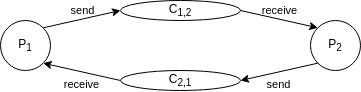
\includegraphics[scale=0.4]{modello_a_rete.png}
    \end{figure}
    \end{block}
\end{textblock*}
\begin{textblock*}{0.3\textwidth}(75mm, 52.5mm)
\begin{block}{}
    \begin{figure}
        \centering
        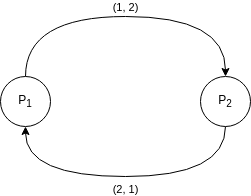
\includegraphics[scale=0.4]{modello_a_rete_digrafo.png}
    \end{figure}
    \end{block}
\end{textblock*}
\end{frame}

\section{Da modello a rete al modello a memoria condivisa}

\begin{frame}{Da modello a rete al modello a memoria condivisa}
    \begin{block}{Perchè convertire un modello a rete in uno a memoria condivisa?}
        \begin{itemize}
            \item I sistemi a memoria condivisa sono di più facile comprensione e offrono una maggiore espressività.
            \item Esistono numerosi algoritmi già sviluppati per i modelli a memoria condivisa.
            \item Il modello a rete simula ed eredita le caratteristiche proprie di un sistema a memoria condivisa.
        \end{itemize}
    \end{block}
\end{frame}

\begin{frame}{Problema del consenso}
    Un insieme di $n$ utenti $U_{i}$ interagiscono con un sistema di n processi $P_{i}$ attraverso un certo modello di comunicazione, ogni utente $U_{i}$ inizializza con un certo valore \textit{v} il processo $P_{i}$ attraverso l'azione $init(v)_{i}$.
    \\[10pt]
    I processi $P_{i}$ interagiranno tra di loro per compiere una scelta unanime di un certo valore $v$ da comunicare agli utenti $U_{i}$ attraverso l'azione $decide(v)_{i}$.
    
    %%%%%%%%%%%%%%% COMMENTO %%%%%%%%%%%%%%%%%%%%%
    \iffalse
    Ogni processo può essere soggetto ad un \textbf{stopping failure}, ovvero può smettere di funzionare senza nessun avviso. Questo può essere modellato attraverso delle azioni di input chiamate $stop_{i}$ le quali non fanno altro che disabilitare ogni azione localmente controllata del processo $P_{i}$. Una esecuzione è detta failure-free se non contiene eventi di $stop$
    \fi
\end{frame}

\subsection{Il problema del consenso}

\begin{frame}{Impossibilità del consenso nel modello a rete}

    Il modello a rete eredita dal modello a memoria condivisa l'impossibilita del consenso.

    \begin{block}{Teorema}
        Dato un qualsiasi sistema asincrono a rete composto da un numero $n \geq 2$ di processi, non esiste un algoritmo che risolva del consenso e garantisca la \textit{1-failure termination}.
    \end{block}
\end{frame}

\begin{frame}{Concetti chiave}
    \begin{itemize}
        \item Fault-tolerance %% Spiegare un evento di stop
        \item I-simulazione
    \end{itemize}
\end{frame}

\begin{frame}{Fault-tolerance}
    Un processo può fallire semplicemente stoppandosi in qualsiasi momento della sua esecuzione. Definiamo questo tipo di fallimento \textbf{stopping failure}. 
    \\[10pt]
    Un fallimento di questo tipo può essere modellato aggiungendo ad ogni processo $P_{i}$ un evento di input chiamato \textit{$stop_{i}$}, questo causa il fallimento del processo cambiandone lo stato e disabilitando tutti i suoi task. 
    \\[10pt]
    Un sistema A interfacciato verso gli utenti U è fault-tolerant rispetto a \textit{f} fallimenti se rispetta la seguente condizione liveness:
    \begin{block}{f-failure termination}
        Per ogni esecuzione del sistema composto $A \times U$ in cui occorrono degli eventi di stop su al più \textit{f} porte, ogni invocazione su una porta non-fallita ha una risposta.
    \end{block}

\end{frame}

\begin{frame}{I-simulazione}
    Un sistema B \textbf{simula} un sistema A se il suo comportamento è indistinguibile per un insieme di utenti esterni U.
    
    \begin{block}{I-simulazione}
        Un sistema B composto da n processi $P_{i}$ con $1 \leq i \leq n$, è una I-simulazione di A se per ogni esecuzione $\alpha$ di B e per ogni collezione di utenti $U_{i}$, esiste una esecuzione $\alpha$' di A con gli stessi utenti per cui:
        \begin{itemize}
            \item $\alpha$ e $\alpha$' sono indistinguibili agli utenti U. % spiegare a voce cosa signigica indistinguibili
            \item per ogni \textit{i} un evento $stop_{i}$ occorre in $\alpha$ se e solo se occorre in $\alpha$'
        \end{itemize}
    \end{block}
    
\end{frame}

\begin{frame}{SimpleSRSim - 1}
\begin{textblock*}{\textwidth}(0mm, 12mm)
    \begin{itemize}
        \item Supponiamo di voler creare un sistema asincrono a memoria condivisa $B$ che ne simuli uno a rete $A$.
        \item Per ogni arco di $A$ che collega due processi $P_i$ e $P_j$, nel sistema B si crea una variabile condivisa $x(i, j)$ modificabile solamente da $P_i$ e leggibile esclusivamente da $P_j$.%\footnote{Si tratta di una variabile condivisa single-reader/single-writer}
        \item Ogni variabile condivisa del tipo $x(i,j)$ contiene una propria coda di messaggi, utile per l’emulazione delle operazioni di base di un sistema a rete.
    \end{itemize}
\end{textblock*}
\begin{textblock*}{0.65\textwidth}(45mm, 50mm)
    \begin{block}{Variabile condivisa single-reader/single-writer}
    \begin{figure}
        \centering
        % Freccia tratteggiata: operazione di lettura
        % Freccia non tratteggiata: operazione di scrittura
        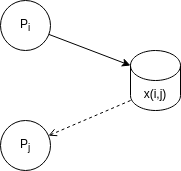
\includegraphics[scale=0.4]{struttura_di_base.png}
    \end{figure}
    \end{block}
\end{textblock*}
\end{frame}

\begin{frame}{SimpleSRSim - 2}
\begin{textblock*}{\textwidth}(0mm, 12mm)
    \begin{itemize}
        \item L'invio del messaggio $m$ dal processo $i$ al processo $j$ viene emulato aggiungendo il messaggio $m$ al fondo della coda contenuta in $x(i, j)$.
        \item Un generico processo $i$ verifica ciclicamente la presenza di eventuali nuovi messaggi ricevuti da un qualche processo $j$ esaminando il contenuto della variabile $x(j, i)$.
        \item L'elaborazione di un generico messaggio $m$ rimane invariata.
    \end{itemize}
\end{textblock*}
\begin{textblock*}{0.4\textwidth}(8mm, 45mm)
\begin{block}{Modello a rete}
\begin{figure}
    \centering
    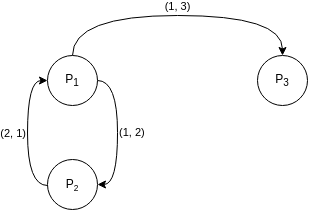
\includegraphics[scale=0.4]{test_sr.png}
\end{figure}
\end{block}
\end{textblock*}
\begin{textblock*}{0.45\textwidth}(65mm, 45mm)

\begin{block}{Modello a memoria condivisa}
\begin{figure}
    \centering
    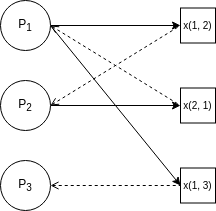
\includegraphics[scale=0.4]{test_sm.png}
\end{figure}
\end{block}
\end{textblock*}
\end{frame}

\begin{frame}{SimpleBCastSim}
    \begin{itemize}[<+->]
        \item In questo caso, per ogni \textit{i} con $1 \leq i \leq n$, il sistema \textit{B} ha una variabile condivisa $x(i)$ a singolo scrittore/multiplo lettore.
        \newline La variabile è scrivibile da \textit{i} e leggibile da tutti i processi (\textit{i} incluso), e contiene una coda di messaggi, inizialmente vuota.
        \item Come con SimpleSRSim, un processo \textit{i} di \textit{B} simula direttamente il processo $P_{i}$ di \textit{A}.
    \end{itemize}
\end{frame}

\begin{frame}{SimpleBCastSim}
    \begin{block}{Broadcast}
        Per simulare un'azione $bcast(m)_{i}$ di $P_{i}$, il processo \textit{i} di \textit{A} aggiunge il messaggio \textit{m} alla fine della coda presente nella variabile \textit{x(i)}.
        \begin{figure}
            \centering
            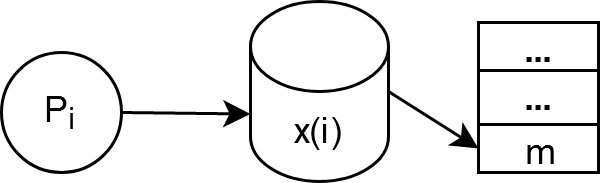
\includegraphics[scale=0.3]{Broadcast.png}
        \end{figure}
    \end{block}
\end{frame}

\begin{frame}{SimpleBCastSim}
    \begin{block}{Ricezione}
        Il processo \textit{i} periodicamente controlla tutte le variabili \textit{x(j)} (inclusa \textit{x(i)}), per verificare se sono presenti dei nuovi messaggi. Se effettivamente ve ne sono, li gestisce allo stesso modo di $P_{i}$.
        \begin{figure}
            \centering
            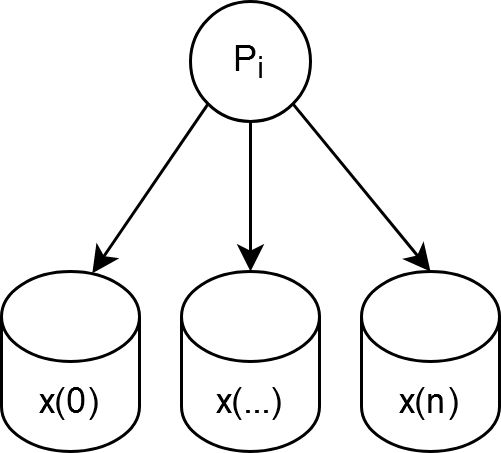
\includegraphics[scale=0.26]{BroadcastReceive.png}
        \end{figure}
    \end{block}
\end{frame}

% SimpSRSim
% SimpBCastSim

\subsection{Equivalenza del modello Send/Receive e il modello Broadcast}

\begin{frame}{Equivalenza tra modello Send/Receive e Broadcast}
    \begin{block}{Teorema}
        Dato un generico sistema asincrono a rete broadcast A esiste un sistema asincrono send / receive B che è una I-simulazione di A.
    \end{block}

    \vspace{0.5cm}

    Data questa equivalenza da ora in poi supporremo di lavorare in sistemi asincroni a rete broadcast, in quanto permettono la stesura di algoritmi più intuitivi e più facilmente dimostrabili.
\end{frame}


\begin{frame}{Impossibilità del consenso nel modello a rete}
    \begin{block}{Dimostrazione}
    \begin{itemize}
        \item Supponiamo per \textbf{assurdo} che esista un algoritmo \texttt{A} in grado di risolvere il problema del consenso in un sistema asincrono a rete broadcast e che garantisca la 1-failure termination.
        \item Per quanto dimostrato è possibile ottenere un algoritmo B per un sistema a modello a memoria condivisa che è un n-simulazione di \texttt{A}.
        \item Pertanto \texttt{B} risolverebbe il problema del consenso garantendo la 1-failure termination. Questo però contraddice il teorema dell'impossibilità del consenso nel modello a memoria condivisa.
    \end{itemize}
    \end{block}
\end{frame}

% Capitolo 21

\section{Una soluzione randomizzata}

\begin{frame}{Una soluzione randomizzata}
    Poichè problema del consenso è di vitale importanze in diversi settori, come ad esempio la gestione di transazioni in database distribuiti; è stato necessario sviluppare degli espedienti:
    \vspace{0.2cm}
    \begin{itemize}
        \item Indebolimento dei requisiti di correttezza
        \item Rafforzamento del modello attraverso:
        \vspace{0.2cm}
        
        %%% ha senso ??? %%%
        \begin{itemize}
            \item \textbf{Utilizzo della randomizzazione}
            \item Failure detection
            \item Consenso su un insieme di valori
            \item Consenso parziale
        \end{itemize}
    \end{itemize}
\end{frame}

\begin{frame}{Requisiti di correttezza}
    Un sistema A risolve il problema del consenso se per ogni collezione di utenti U garantisce:
    \begin{itemize}
        \item \textbf{Well-formedness}: ogni interazione tra il sistema ed utenti $U_{i}$ è ben formata:
        \begin{itemize}
            \item Non contiene azioni ripetute di \textit{init},
            \item Non contiene azioni ripetute di \textit{decide},
            \item Ogni \textit{decide} è preceduto un \textit{init}.
        \end{itemize}
        \item \textbf{Agreement}: Tutti i valori di decisione sono uguali.
        \item \textbf{Validity}: Se tutte le azioni di \textit{init} danno in input lo stesso valore \textit{v}, allora l'unico valore che può essere deciso è \textit{v}.
        \item \textbf{Failure-free termination}: In ogni esecuzione failure-free in cui un \textit{init} è stata fatta su ciascuna porta, un evento \textit{decide} viene fatto su tutte le porte.
    \end{itemize}
\end{frame}

\begin{frame}{Requisiti di terminazione}
    Un sistema A composto da n processi $P_{i}$ è \textit{fault-tolerant}, rispetto a \textit{f} ($0 \leq f \leq n$) fallimenti, se soddisfa la seguente proprietà di terminazione: 
    \begin{block}{f-failure termination}
    In ogni esecuzione fair in cui degli eventi di \textit{init} occorrono su tutte le porte, se ci sono al più \textit{f} eventi di \textit{stop}, allora un evento di \textit{decide} occorre su tutte le porte non-fallite. 
    \end{block}
    % potremmo parlare di 1-failure termination e n-failure termination
\end{frame}

\subsection{Algoritmo di BenOr}
\begin{frame}{Algoritmo di BenOr}
    \begin{itemize}
        \item L'algoritmo di BenOr funziona con $n > 3f$ processi e con l'insieme di valori di scelta $V = \{0, 1\}$.

        \item Ogni $P_{i}$ esegue una serie infinita di \textbf{stage} numerati in maniera incrementale ed ognuna di essa è divisa in due \textbf{round}.

        \item I processi nei vari stage si scambiano messaggi i quali contengono:
            \begin{itemize}
                \item un tag che può essere o R (Report) o P (Propose);
                \item un numero che indica lo stage corrente, indicato con $s$;
                \item un valore definito nel round indicato con $v$.
            \end{itemize}

        \item L'algoritmo termina l'esecuzione degli stage finché non si presenta una $decide(v)_{i}$.
    \end{itemize}
\end{frame}

\begin{frame}{Algoritmo di BenOr - Inizializzazione}
    \begin{itemize}
        \item Ogni processo $P_{i}$ ha due variabili locali $x$ e $y$ inizializzate a $null$.

        \item All'occorrenza di un input $init(v)_{i}$ sul processo $P_{i}$ viene assegnato ad $x$ il valore $v$ ($v \in V$).

        \item La numerazione degli stage inizia con il valore 0 e viene incrementato all'inizio di ogni round 1.
    \end{itemize}
\end{frame}


\begin{frame}{Algoritmo di BenOr - Round 1}
    \begin{itemize}
        \item $P_{i}$ invia in broadcast agli altri processi un messaggio della forma \mbox{(R, s, x)}.

        \item Successivamente attende di ricevere messaggi (R, s, *) da n - f processi\footnote{( può essere 0 o 1)}.

        \item Se tutti i messaggi ricevuti hanno lo stesso valore $v$ allora salva nella variabile $y$ il valore $v$.

        \item altrimenti salva in $y$ il valore null.

    \end{itemize}
\end{frame}


\begin{frame}{Algoritmo di BenOr - Round 2}

    \begin{itemize}
        \item $P_{i}$ invia in broadcast agli altri processi un messaggio della forma \mbox{(P, s, y)}.

        \item Successivamente attende di ricevere messaggi (P, s, *) da n - f processi\footnote{( può essere 0 o 1 o null)}.

        \item Se tutti i messaggi ricevuti hanno lo stesso valore $v$ e $v$ diverso da null allora salva in $x$ il valore $v$ ed esegue l'azione $decide(v)_{i}$.

        \item altrimenti Se almeno $n - 2f$ messaggi ricevuti hanno lo stesso valore $v$ e $v$ diverso da null allora salva in $x$ il valore $v$.

        \item altrimenti viene assegnato ad $x$ un valore scelto randomicamente dall'insieme V.
    \end{itemize}
\end{frame}

% dimostrazione benor 

% simulazione benor

\end{document}
